% !TEX root = ../main.tex
\chapter{Vigra Graph Library} \label{ch:vigra_graph_lib}


\section{Choosing the right Graph API}

Argue why we choose lemon api 

\section{Implementation}\label{sec:vigra_graph_lib_impl}

\section{Graph API's}\label{sec:graph_apis}

    \subsection{LEMON Graph API's}\label{sec:lemon_graph_apis}
    Give brief overview of lemons graph api 
    \subsection{BOOST Graph API's}\label{sec:boost_graph_apis}
    Give brief overview of boost graph api
    \subsection{VIGRA Graph API}
    Explain why which api is used and how it is extended


\section{Graphs}


\subsection{Grid Graph}

\missingfigure{show grid graph here}

    \lstinline{vigra::GridGraph<DIM,DIRECTED_TAG>}

\subsection{Adjacency List Graph}

\subsection{Merge Graph}
To implemented structured clustering algorithms (see \cref{???}) we
need a graph which supports the contraction of edges.
Also a mechanism to merge node and edge features is needed.
Experiments suggest that the edge contraction is more expensive
than feature merging an can even be a bottleneck for huge 3D data 
(see \cref{???} ).
Therefore it is crucial to implemented the MergeGraph (MG) very carefully.
\begin{figure}
    \centering
    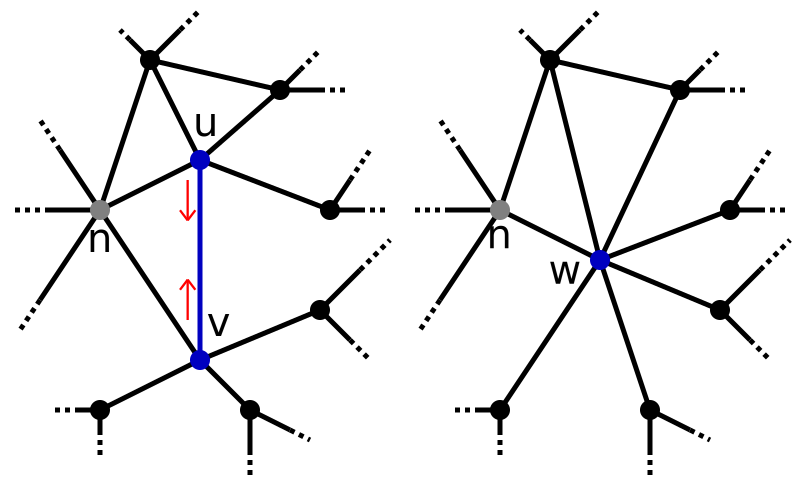
\includegraphics[width=0.35\textwidth]{fig/contraction.pdf}
    \caption{ Schematic edge contraction: Node $u$ and $v$ is merged into node $w$.
        Note the gray node $n$ which is connected to $u$ and $v$.
        After the contraction, edges $\{ n,u\}$ and $\{ n,v\}$ are also merged into 
        a single edge $\{ n, w\}$ 
    }
    \label{fig:figlabel}
\end{figure}

   

\begin{center}
    \begin{tikzpicture}
        \umlclass[template=Graph]{MergeGraphAdpator}
        {
            \\// union find data structures                     \\
            - edgeUfd               : IterablePartiton          \\
            - nodeUfd               : IterablePartiton          \\ 
            - nodesAdjacency        : AdjacencySetVector        \\

            \\// callbacks                                      \\
            - mergeNodeCallBacks    : MergeNodeCallBackVector   \\
            - mergeEdgeCallBack     : MergeEdgeCallBackVector   \\
            - eraseEdgeCallBack     : EraseEdgeCallBackVector   \\
        }
        {
            \\// LEMON API for undirected graphs                \\
                $\ldots$                                        \\
            \\// register callbacks                             \\ 
            + registerMergeNodeCallBack(f : MergeNodeCallBack)  \\
            + registerMergeEdgeCallBack(f : MergeEdgeCallBack)  \\
            + registerEraseEdgeCallBack(f : EraseEdgeCallBack)  \\

            \\// modify graph                                   \\
            + contractEdge(edge : Edge)     : Node              \\

            \\// find representatives                           \\
            + reprNode(node : Node)         : Node              \\
            + reprEdge(edge : Edge)         : Edge              \\ 

            \\// get base graph                                 \\
            + graph()                       : Graph             \\
        } 
    \end{tikzpicture}
\end{center}



\begin{center}
    \begin{tikzpicture}
        \umlclass[template=MergeGraph]{ClusterOperatorInterface}
        {

        }
        {
            \\// contract next edge and get weight              \\
            + contractionEdge(edge : Edge)         : Edge       \\ 
            + contractionWeight(edge : Edge)       : Edge       \\
            \\// get base graph                                 \\
            + mergeGraph()                  : MergeGraph        \\
        } 
    \end{tikzpicture}
\end{center}


\begin{center}
    \begin{tikzpicture}
        \umlclass[template=ClusterOperator]{HierarchicalClustering}
        {

        }
        {
            + cluster()                     : void        \\
            + reprLabels(nodeMap : NodeMap) : void        \\      
        } 
    \end{tikzpicture}
\end{center}


   We propose and implemented the following design:
   \begin{compactitem}
       \item  A base graph is attached to a merge graph  and  a merge graph will
            always ``view'' to
       \item  Union find data structure for nodes
       \item  Union find data structure for edges
   \end{compactitem}



   \lstinline{vigra::MergeGraphAdaptor<DIM,DIRECTED_TAG>}

\subsection{Region Adjacency Graph}

    \missingfigure{show region adjacency graph here}

\section{Graph Algorithms}

    \section{Multicut}

    \section{Hierarchical Clustering}

    \section{Mst Algorithms}

    \section{Watershed Algorithms}

    \section{Smoothing Algorithms}





\section{Python}

On the python side, we want node-maps,edge-maps and arc-maps to be stored 
as numpy arrays for ??? reasons.:
\begin{compactitem}
    \item Numpy arrays are the standard for storing multidimensional data in python.
    The fast C implementations and a vectorized API of numpy make it very easy to write 
    fast python code within a few lines.
    Virtually any python user will be familiar with the numpy API and therefore it 
    seems to be natural to store graph maps within numpy arrays.
    \item Vigra provides an mechanism to pass numpy arrays to C++.
    Therefore no new mechanism needs to be implemented to transfer graph
    maps from python to C++.
    This will not only simplify writing extension for the new vigra graph api,
    but also it will reduce the glue code since we can use well tested existing
    solutions.
    \item New algorithms might be implemented in pure python with a mix of
    existing numpy functions and new functions provided within vigras graph api.
    As a proof of concept we implemented ??? in pure python with vigras
    fresh graph api in \cref{???}.
\end{compactitem}

On the C++ side, numpy arrays are stored in MultiArrayViews.
Since API of MultiArrayViews \cite{software_vigra_multiarray_api} does
not implemented the API  of LEMON graph maps (e.g. node-maps,edge-maps and arc-maps).
 

\begin{lstlisting}[language=python]
vigra.graphs.foobar(graph,nodeFeatures)
\end{lstlisting}
\section{Some Tikz stuff}




\begin{lstlisting}[language=c++]
static NumpyAnyArray ConverterStruct::foobar(
    const Graph & graph , 
    const typename PyNodeMapTraits<Graph, UInt32>::Array & nodeArray
){
    typename PyNodeMapTraits<Graph, UInt32>::Map nodeArrayMap(graph,nodeArray)

    // code using LEMON Map Api 
}
\end{lstlisting}
